\section{Introduction}\label{sec:intro}
\vspace{-10pt}
\begin{quote} {\em
... today's researchers must consume ever higher volumes 
of numbers that gush, as if from a fire hose ... 
}
\end{quote}
\vspace{-7 pt}
\noindent \hspace{80pt} --- R.M. Friedhoff and T. Kiely
\smallskip

Data analysts must sift through huge volumes of data
looking for valuable data-specific insights, trends, or anomalies.
This process involves selecting the ``right'' subset of the data,
and the ``right'' way to view it, so that the ``insights'' become apparent.
Moreover, the process is often ad-hoc and consumes a lot of the analyst's time.
Our vision is that {\em some especially cumbersome aspects} of this search 
for interesting insights can be automated.

To illustrate, consider the following interactive exploration workflow,
which we believe is often used in practice.

\noindent 
{\em Step (1):} First, the analyst poses a relational query 
to extract some subset of data they are interested in exploring.
For example, the analyst may select all records associated with
``stapler'' products.





\noindent {\em Step (2):} Then, the analyst considers several candidate views 
over this subset of data, formed by, say, aggregation and grouping;
the analyst must study all of these views one by one.
For example, one view may be total stapler sales by year,
while another view may be the quantity in stock by sales region.
Since these views have two-attributes each, we can view them
as 2-dimensional graphs. 
For example, Figure 1(a) may be the stapler sales (y-axis) by year (x-axis),
while Figure 1(c) may be the quantity (y-axis) by region (x-axis).
(Figures 1(b) and 1(d) are discussed below.)




\noindent {\em Step (3):} Next, the analyst steps 
through each view, and decides which views are ``interesting.''
This of course is the critical and time-consu\-ming step.
What makes a view like Figure 1(a) interesting or not?
Well, it all depends on the application semantics
and what we are comparing against.
For example, Figure 1(a) shows decreasing sales over time.
If we are in a recession and all product sales are down then this observation
is not very interesting. However, say that Figure 1(b) shows
the aggregate (all) product sales over the same time periods.
Then the stapler sales view goes against the general trend: 
overall sales are up, but stapler sales are going down.
In this case, the view is {\em potentially} ``interesting''
because it depicts a trend in the subset of data
that the analyst is interested in (i.e., stapler-related data)
that {\em deviates} from the trend in the overall data.
Of course, the analyst must decide if this deviation 
is truly an insight for this application.
Even so, our key insight is that we may be able to 
{\em identify and highlight to the analyst potentially interesting views 
using automated mechanisms based on deviation}.
By doing so, we eliminate the laborious process
of stepping through all possible views that the analyst currently 
performs.
Once we recommend potentially interesting views, we can let the analyst
make the final decision.

\pgfmathdeclarefunction{gauss}{2}{%
  \pgfmathparse{1/(#2*sqrt(2*pi))*exp(-((x-#1)^2)/(2*#2^2))}%
}

\pgfplotsset{ticks=none}

\begin{figure}[htp]
  \centering
  \vspace{-10pt}
    \subfigure[]
    {\begin{tikzpicture}[scale = 0.15]
      \begin{axis}[
      axis lines=center,
      axis on top=true,
      enlargelimits=0.15,
      symbolic x coords={mod2,mod3,mod5,mod7,mod11,mod13,mod17,mod19,mod23},
      ]
    \addplot[draw=red, ultra thick] coordinates 
      { (mod2,80) (mod3,79.7961) (mod5,75)
        (mod7,73) (mod11,69) (mod13,65)
        (mod17,60) (mod19,53) (mod23,50)};
    \end{axis}
    \end{tikzpicture}}
    \subfigure[]
    {\begin{tikzpicture}[scale = 0.15]
    %   \begin{axis}[
    %   xmin=0, xmax=1.5,
    %   ymin=0, ymax=1.5,
    %   axis lines=center,
    %   axis on top=true,
    %   domain=0:1,
    %   ]
    % \addplot [mark=none,draw=red,ultra thick] {x};
    \begin{axis}[
      axis lines=center,
      axis on top=true,
      enlargelimits=0.15,
      symbolic x coords={mod2,mod3,mod5,mod7,mod11,mod13,mod17,mod19,mod23},
      ]
    \addplot[draw=red, ultra thick] coordinates 
      { (mod2,80) (mod3,87) (mod5,95)
        (mod7,98) (mod11,105) (mod13,115)
        (mod17,120) (mod19,123) (mod23,129)};
    \end{axis}
    \end{tikzpicture}}
    \subfigure[]
    {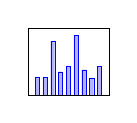
\begin{tikzpicture}[scale = 0.15]
%       \begin{axis}[every axis plot post/.append style={
%   mark=none,domain=-2:3,samples=50,smooth}, % All plots: from -2:2, 50 samples, smooth, no marks
%   axis x line*=bottom, % no box around the plot, only x and y axis
%   axis y line*=left, % the * suppresses the arrow tips
%   enlargelimits=upper] % extend the axes a bit to the right and top
%   \addplot {gauss(0,0.25)};
% \end{axis}
    \begin{axis}[
      ymin=70, ymax=120,
      axis on top =true,
      ybar,
      enlargelimits=0.15,
      symbolic x coords={mod2,mod3,mod5,mod7,mod11,mod13,mod17,mod19,mod23},
      ]
    \addplot coordinates 
      { (mod2,80) (mod3,79.7961) (mod5,114.4597)
        (mod7,85) (mod11,90.5600) (mod13,120)
        (mod17,87) (mod19,79) (mod23,90)};
    \end{axis}
    \end{tikzpicture}
    }
    \subfigure[]
    {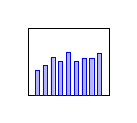
\begin{tikzpicture}[scale = 0.15]
      \begin{axis}[
      ybar,
      ymin=70, ymax=100,
      enlargelimits=0.15,
      symbolic x coords={mod2,mod3,mod5,mod7,mod11,mod13,mod17,mod19,mod23},
      ]
    \addplot coordinates 
      { (mod2,80) (mod3,82.7961) (mod5,87.4597)
        (mod7,85) (mod11,90.5600) (mod13,85)
        (mod17,87) (mod19,87) (mod23,90)};
    \end{axis}
    \end{tikzpicture}
    }
    \vspace{-13pt}
    \caption{Views (a), (b): Sales over Time. (c), (d): Quantity by Region.}\label{fig:plots}
    \vspace{-12pt}
 \end{figure}

Figures 1(c) and 1(d) illustrate a different type of deviation.
The first figure shows the distribution of staplers
across regions, while the second figure shows the
overall product distribution.
Again, the stapler view does not follow the general trend:
the regions that have the most staplers are not the larger regions
that have most product in stock.
The analysis must decide if this observation is interesting:
perhaps the region that has many staplers is near
the world-famous stapler-gun-wrestling contest,
in which case the observation is expected.
But perhaps there is a problem with the product shipping strategy,
in which case the deviation is very important.
% In this example as well, there is a deviation between
% the distribution in the subset of data that the analyst is interested in,
% and the rest of the data in the database.
% Thus, our goal is to automate the search for views that are {\em potentially}
% interesting, and to then let the analyst make the final decision.









\begin{figure}[t!]
\vspace{-15pt}
\begin{center}
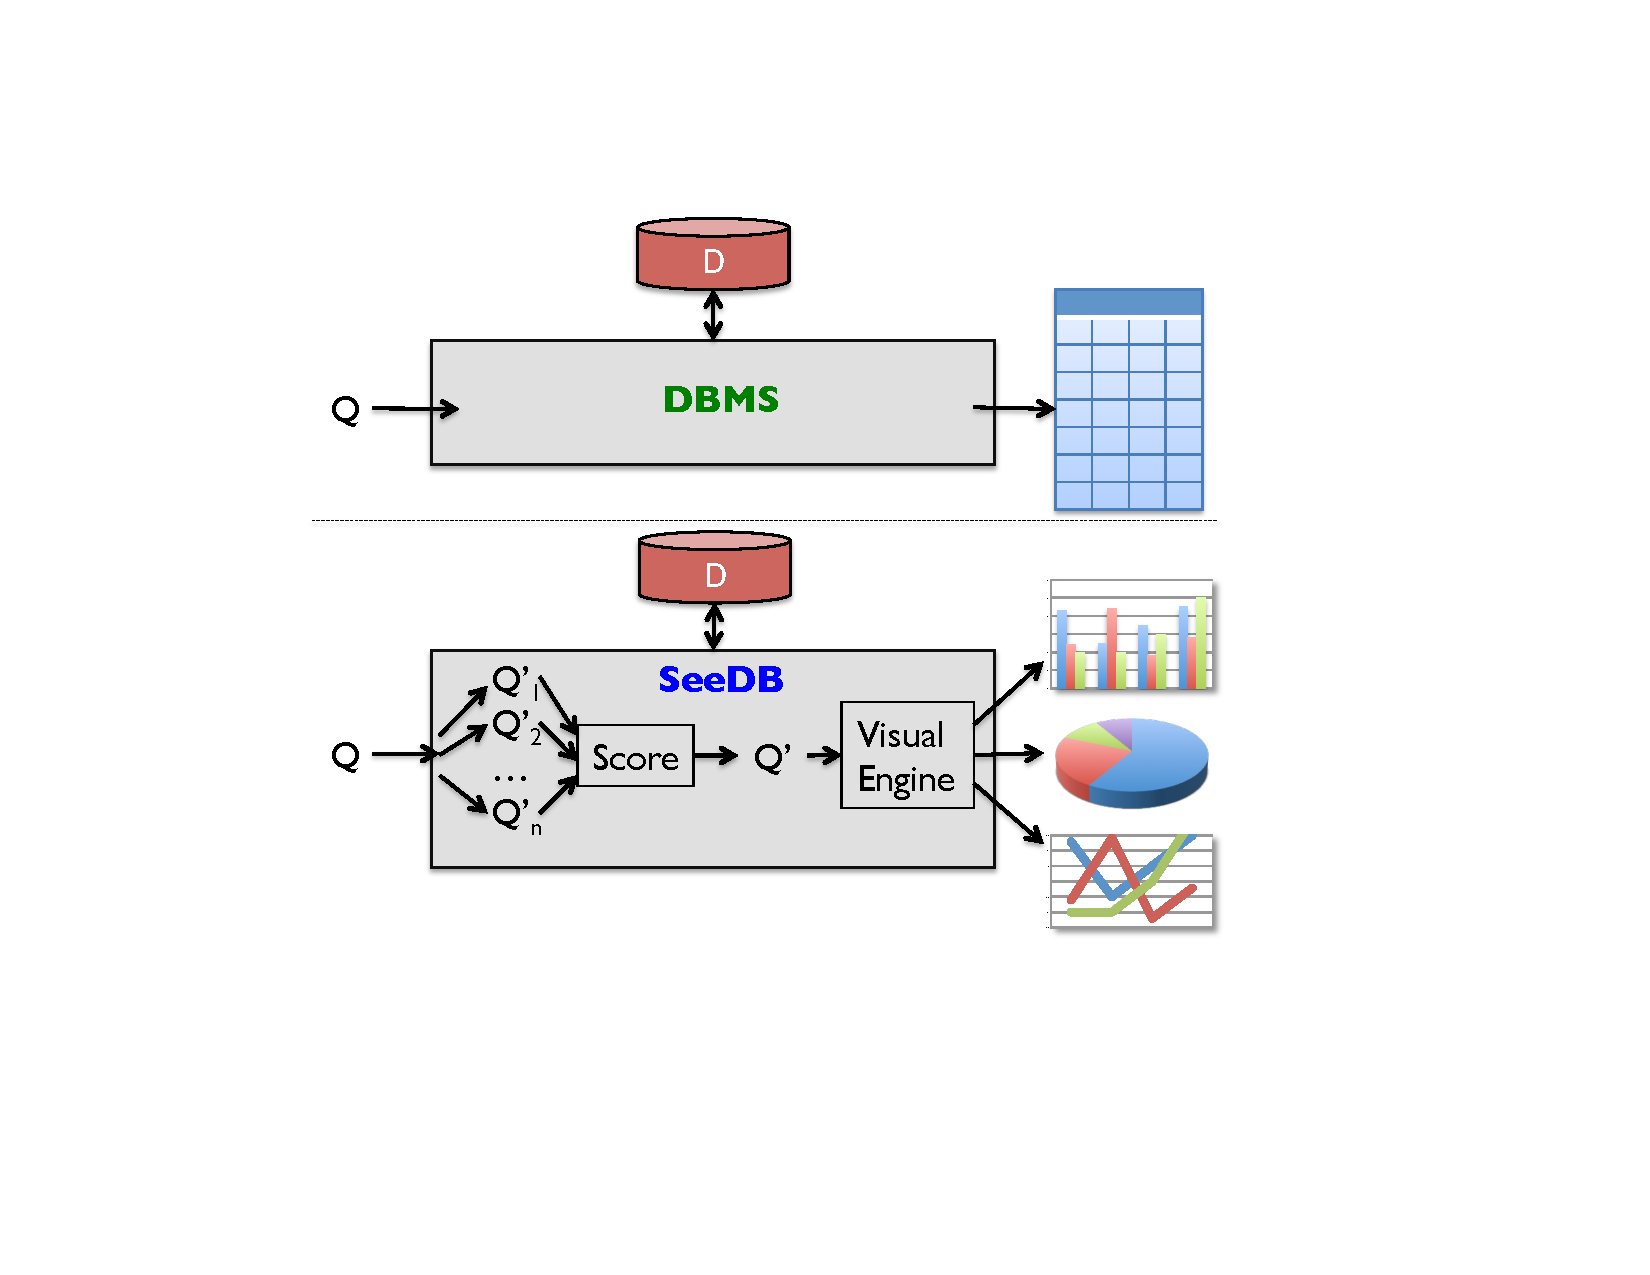
\epsfig{file=Images/comparison-diagram.pdf, width=1.5in, trim=3in 2.5in 3in 1in}
\end{center}
\vspace{-10pt}
\caption{\SeeDB\ Comparison with regular DBMS\label{fig:comparison} (The workflow for \SeeDB\ is only conceptual and need not happen in that order.)}
\vspace{-15pt}
\end{figure}

In this vision paper, we sketch our design for a new data base management system
(DBMS), \SeeDB, that automates the especially laborious 
aspects of the search for useful data insights.
Figure 2 depicts \SeeDB, together with a conventional DBMS.
In the conventional system, the user or analyst submits a query $Q$
and obtains data subsets.
Thus, conventional systems do not provide any means for the analyst 
to get intuitive visual insights directly.
In \SeeDB, the analyst also submits a query, but instead
automatically obtains views (or visualizations) of the query result
that are potentially of interest.
As illustrated in our examples,
these visualizations help the
analyst quickly interpret and understand specific
``interesting/useful'' aspects of the query result.
Thus, with \SeeDB, we fundamentally modify the
query-result paradigm of databases: \SeeDB\ is provided a query $Q$,
and outputs visualizations of interesting aspects
of $Q$.

Given a database and a query $Q$, \SeeDB\ considers a space of views 
$Q_1', \ldots, Q_n'$ that
are generated by adding to $Q$ additional relational operators, 
such that the results can be readily visualized 
(via the visual engine, depicted in Figure~\ref{fig:comparison}).
For instance, one possibility in our Staplers example was to 
add a group by and an aggregation giving a view corresponding to total sales of Staplers per region. 
We call these views $Q_1', \ldots, Q_n'$ the {\em discriminating views}.
To decide if a discriminating view is interesting, \SeeDB\ compares it
to the equivalent view obtained from the full database, using the
same operators.
For comparing the two views, \SeeDB\ 
uses a set of functions that captures how much the first view {\em deviates}
from the second.  
Prior work in the visualization community has identified
several functions for this purpose; however an important
issue is the feasibility of computing such functions on 
large databases.
These functions capture the deviations illustrated in
our initial example (e.g., different slopes), and draw
from existing functions that compare value distributions
(e.g., earth movers function).
Of course, \SeeDB\ is not tied to any particular function(s),
and allows the analyst to override the defaults using 
their own functions.
We say that \SeeDB\ computes the {\em utility} of discriminating 
view when it compares the discriminating view against the same
view on the database.

\techreport{Even if \SeeDB\ limits the discriminating views considered, the cost of computing utilities may be prohibitive. Thus, we will also suggest techniques for improving performance. For example, it may be possible to reuse some of the computations from evaluating one view, in evaluating the utility of another view. A different avenue for improving performance, is to provide approximate results, either by reducing the size of a view, or by computing its utility approximately.}



% Since the space of possible views that \SeeDB must explore is huge,
% for tractability the space must be constrained.
% Here we will suggest the following constraints,
% which we believe can be relaxed in the future.
% We focus on a database with a traditional star schema,
% and a query $Q$ on the fact table.
% (We illustrate these terms, as well as other terms 
% in this paragraph, in the example below.)
% \SeeDB considers 2-attribute views that are generated by adding to $Q$
% a single aggregation and group-by operator.
% We call these views the {\em discriminating views}.
% To decide if discriminating view $V$ is interesting, \SeeDB compares it
% to the equivalent view $V_D$ obtained from the full database, using the
% same aggregation and group-by operator.
% To determine if $V$ and $V_D$ are significantly different, \SeeDB uses
% a set of analyst-provided comparison functions.
% These functions capture the differences illustrated in
% our initial example (e.g., different slopes), and draw
% from existing functions that compare value distributions
% (e.g., earth movers function).
% We say that \SeeDB computes the {\em utility} of $V$
% when it compares it against $V_D$.

% Even if \SeeDB limits the discriminating views considered,
% the cost of computing utilities may be prohibitive.
% Thus, we will also suggest techniques for improving 
% performance. For example, it may be possible to reuse some of the
% computations from evaluating one view, in evaluating the utility of another view.
% A different avenue for improving performance, is to
% provide approximate results, either by reducing the size of a view,
% or by computing its utility approximately.

Our next example is a more detailed version of the previous example,
and clarifies the terms introduced.

\begin{example}\label{example}
\vspace{-10pt}
We focus on a database with a traditional star sch\-ema.
We operate on a single fact table $D$, containing information
about sales. The schema of $D$ comprises three dimension
attributes: \att{Product}, \att{Location}, and \att{Year}, and
one measure attribute: \att{Sales}.

Let us assume our analyst has entered a query with a
single selection predicate:
$Q \equiv \sigma_{(\att{Product = Staplers})}$.
The result contains too many tuples to examine individually, and
hence the analyst has to rely on some appropriate visualization in order
to glean interesting insights about the overall query result.

\SeeDB\ searches over all possible discriminating views that
can be obtained by adding a single aggregate and group by operator.
We initially focus on these two-attribute discriminating views
because they are easy to visualize using histograms or line plots.
(\SeeDB\ also considers more general views.)
One of these queries is 
$Q_1' = R_1(Q)$ where $R_1 \equiv \gamma_{\att{Location, sum(Sales)}}$.
This query tracks the sum of \att{Sales} over \att{Location}.
A possible result, $R_1(Q(D))$, is the discriminating view
shown in the top part of Table 2.
Another possible query is $Q_2' = R_2(Q)$, where $R_2 \equiv
\gamma_{\att{Year, sum(Sales)}}$, tracking the sum of
\att{Sales} over \att{Year}.
The bottom part of Table 2 shows a possible result of this
second view.


The next step is to score each view based on its utility, i.e., its
ability to show an interesting property of the query result. For this
purpose, \SeeDB\ obtains aggregate statistics for
\att{Sales} for \att{Location} and \att{Year} for the original full database.
(As we will see later, there
are interesting optimization opportunities if we can integrate this
step with the processing of $Q$.)
Table 1 shows the full database aggregates, i.e., $R_1(D)$ and $R_2(D)$
corresponding to our sample views.
(Note the missing $Q$.)
For the \att{Location} attribute, both $R_1(D)$ and $R_1(Q(D))$
have similar distributions.
(The fact that sales are uniformly lower in $R_1(Q(D))$ is not
surprising since $R_1(Q(D))$ only considers a fraction of the data.)
However, notice that the
distribution across \att{Year}s is very different for tuples
satisfying \att{Product = `Staplers'}. That is, demand for
\att{`Staplers'} seems to have not gone up, unlike the other products.
This unexpected behavior will be detected by \SeeDB\ when it
computes the utility of $R_2(Q)$, and hence $R_2(Q)$
(and not $R_1(Q)$) will be suggested to the analyst for further human evaluation.

\vspace{-10pt}
\end{example}


\begin{table}
{\scriptsize \center
\vspace{-10pt}
\begin{tabular}{|c|c|c|c|}
\hline
\multicolumn{4}{|c|}{\att{Location} Aggregates: $R_1(Q(D))$ } \\ \hline
Boston: 30 & Seattle: 40 & New York: 40
& San Francisco: 90  \\
\hline
 \hline 
\multicolumn{4}{|c|}{\att{Year} Aggregates: $R_2(Q(D))$} \\ \hline
2009: 50 & 2010: 40 & 2011: 60 & 2012: 50  \\
\hline
\end{tabular} 

\vspace{-10pt}
\caption{Aggregates for \att{Product = `Staplers'} \label{tab:new-agg}}
}
\end{table}


\begin{table}
\vspace{-10pt}
{\scriptsize \center

\begin{tabular}{|c|c|c|c|}
\hline
\multicolumn{4}{|c|}{\att{Location} Aggregates: $R_1(D)$} \\ \hline
Boston: 300 & Seattle: 300 & New York: 300
& San Francisco: 700  \\
\hline
 \hline 
\multicolumn{4}{|c|}{\att{Year} Aggregates: $R_2(D)$ } \\ \hline
2009: 100 & 2010: 200 & 2011: 500 & 2012: 800  \\
\hline
\end{tabular} 

\vspace{-10pt}
\caption{Original Aggregates\label{tab:original-agg}}
}
\vspace{-18pt}
\end{table}

\noindent Thus, there are several technical challenges that need to be addressed:

\begin{denselist}

\item For a given query, $n$, the total number of discriminating views, is
likely to be very large to explore exhaustively and precisely. Even if we
restrict ourselves to views that append a group-by and an aggregation, the
number of choices depends on the number of aggregation methods and group-by
attributes. Generating each of $R_1(Q(D)),$  $\ldots,$ $R_n(Q(D))$, scoring them
on utility, and then picking the best one is certainly not feasible for most
databases. Thus, we need mechanisms to prune the space of views and compute
their utility approximately. This approach is reminiscent of how a query
optimizer costs and prunes candidate execution plans, except that the objectives
are different and hence may require different cost models and data statistics.
In addition, given that the end result is consumed by an analyst, it may be
preferable to recommend a visualization with lower utility but also lower cost
to generate. This option creates a bi-criterion optimization problem, where
possible visualizations may trade off between utility and cost.

\item Generating and scoring the discriminating views $R_i(Q(D))$ one-by-one may
miss interesting optimization opportunities: First, we may share computation
between discriminating views.  For example, the results of two views with
different aggregates but the same group-by may be computed together in one
query, followed by projecting out to reveal the two individual views.  Second,
by evaluating the discriminating views in a deliberate order, we may be able to
prune views with low utility (without evaluation) that are definitely not going
to be recommended to the analyst.

\item Since visualizations tend to convey approximate information, e.g., a trend
in a line plot may be more important than knowing the exact coordinates of each
point, we can introduce approximations as part of \SeeDB.  Thus, the utility of
a discriminating view may be computed approximately but efficiently, and the
recommended discriminating views can be populated with approximate results,
based on synopses of the base data or of the query result, that can be generated
much more efficiently.

\end{denselist}

\noindent Over the past few years, there has been a significant
effort from the visualization community to provide interactive tools
for data analysts. In particular, tools such as ShowMe, Polaris, and
Tableau~\cite{DBLP:journals/cacm/StolteTH08,
  DBLP:journals/tvcg/MackinlayHS07} provide a canvas for data analysts
to manipulate and view data, tools such as
Wrangler~\cite{DBLP:conf/chi/KandelPHH11} allow data analysts to
transform and clean data, and tools such as
Profiler~\cite{DBLP:conf/avi/KandelPPHH12} allow users to visualize
simple anomalies in data.  However, unlike \SeeDB, these tools have
little automation; in effect, it is up to the analyst to generate a
two-column result (like the result of the discriminating view)
to be visualized.

In this paper, we present our goals formally, and then present our initial design for \SeeDB, along with the underlying challenges.